\documentclass[10pt,tikz,border=1mm]{standalone} 
\usepackage{mathpazo}
\usepackage[T1]{fontenc}
\usetikzlibrary{calc,arrows.meta}
\def\centerarc[#1]#2(#3)#4(#5:#6:#7){%
	% \centerarc[draw options](center)(initial angle:final angle:radius)
	\draw[#1] ($(#3)+({#7*cos(#5)},{#7*sin(#5)})$) arc (#5:#6:#7);
}
\tikzstyle{dot}=[circle,fill=black,inner sep=1pt]
\begin{document}
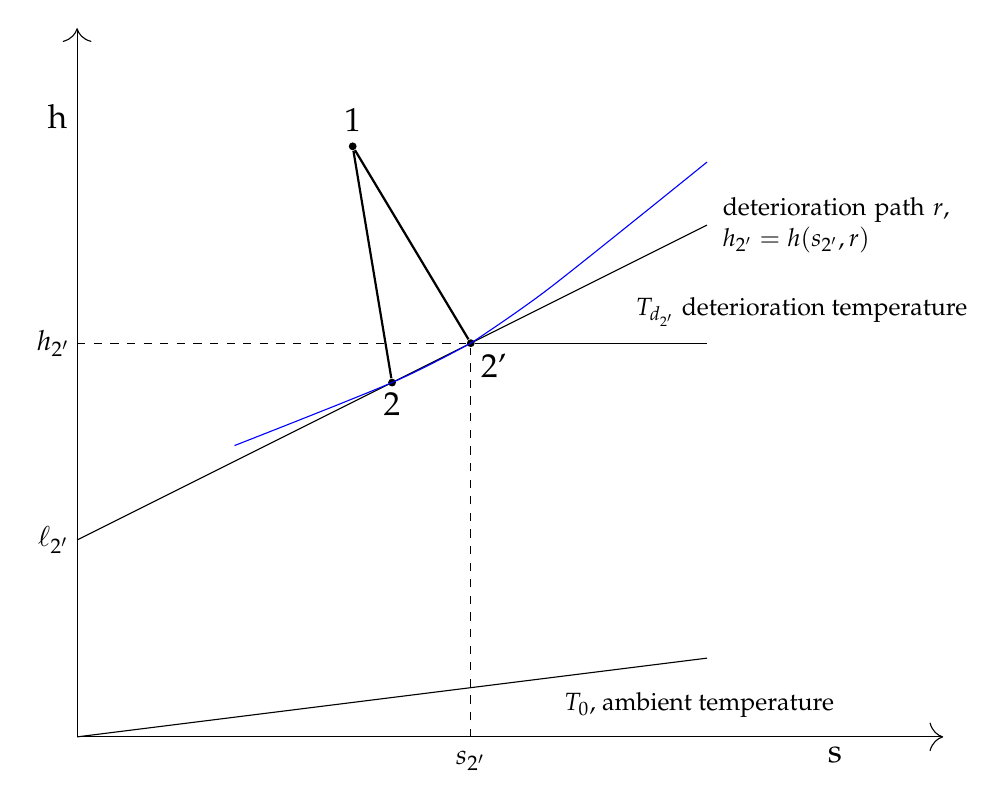
\begin{tikzpicture}[font=\large]
	%\draw[step=1cm,black!20,very thin] (0,0) grid (12,10);
	\draw[-{>[scale=2]},thin] (0,0) -- node[left,very near end]{h} (0,9);
	\draw[-{>[scale=2]},thin] (0,0) -- node[below,very near end]{s} (11,0);
	\node [dot] (P) at (5,5) {};
	\node [dot]  (B) at (4,4.5) {};
	\node[dot,label={above:1}] (A) at (3.5,7.5) {};
	\draw (0,2.5) -- (8,6.5);
	\draw[blue] plot [smooth] coordinates {(2,3.7) (B) (P)};
	\draw[blue] plot [smooth] coordinates {(P) (6,5.7) (8,7.3)};
	\draw[thin,dashed] (0,5) -- (P);
	\draw[thin,dashed] (5,0) -- (P);
	\draw[thick] (A) -- (P) node[below right] {2'};
	\draw[thick] (A) -- (B) node[below] {2};
	\draw (P) -- (8,5);
	\draw (0,0) -- (8,1);
	\centerarc[thin,blue] (0,0) (0:7.2:6cm);
	\centerarc[thin,blue] (P) (0:27:2cm);
	\node[font=\small] at (9.2,5.4) {$T_{d_{2'}}$~deterioration temperature};
	\node[font=\small,text width=3cm] at (9.7,6.5) {deterioration path $r$, $h_{2'}=h(s_{2'},r)$};
	\node[font=\small] at (7.9,0.4) {$T_0$,~ambient temperature};
	\node[font=\normalsize] at (-0.3,2.5) {$\ell_{2'}$};
	\node[font=\normalsize] at (-0.3,5) {$h_{2'}$};
	\node[font=\normalsize] at (5,-0.3) {$s_{2'}$};
\end{tikzpicture}
\end{document}